\documentclass[11pt,a4paper]{article}

\newcommand{\doctitle}{Storm-Gauge Forward Model (MKM-SG-001)}
\newcommand{\docsubtitle}{Wolfram Oracle Benchmark of the Code and its v1.3 Document}
\newcommand{\docversion}{0.1}
\newcommand{\docdate}{04-November-2026}
\newcommand{\docauthor}{David K Kelly}

% MKM Research Labs — Shared Document Header
% Usage: % MKM Research Labs — Shared Document Header
% Usage: % MKM Research Labs — Shared Document Header
% Usage: \input{../shared/mkm_header}  (before \begin{document})
%
% Required commands before \input:
%   \newcommand{\doctitle}{...}
%   \newcommand{\docsubtitle}{...}
%   \newcommand{\docversion}{1.0}
%   \newcommand{\docdate}{13-February-2026}
%   \newcommand{\docauthor}{David K Kelly}

% ─── Packages ───────────────────────────────────────────────────────────────
\usepackage[utf8]{inputenc}
\usepackage{amsmath,amsfonts,amssymb}
\usepackage{listings}
\usepackage{color,xcolor}
\usepackage{graphicx}
\usepackage{hyperref}
\usepackage[toc,page]{appendix}
\usepackage{tabto}
\usepackage{float}
\usepackage{comment}
\usepackage[en-GB]{datetime2}
\usepackage{setspace}
\usepackage{subcaption}
\usepackage{booktabs}
\usepackage{longtable}
\usepackage{adjustbox}
\usepackage{enumitem}
\usepackage{fancyhdr}
\usepackage{lastpage}

% ─── Page geometry ──────────────────────────────────────────────────────────
\onehalfspacing
\usepackage{geometry}
\geometry{a4paper, total={170mm,247mm}, left=20mm, top=25mm, bottom=25mm}

% ─── Headers and footers ───────────────────────────────────────────────────
\pagestyle{fancy}
\fancyhf{}
\fancyhead[L]{\small\textcolor{gray}{MKM Research Labs}}
\fancyhead[R]{\small\textcolor{gray}{\doctitle{} --- v\docversion}}
\fancyfoot[C]{\small\textcolor{gray}{CONFIDENTIAL}}
\fancyfoot[R]{\small\textcolor{gray}{Page \thepage\ of \pageref{LastPage}}}
\renewcommand{\headrulewidth}{0.4pt}
\renewcommand{\footrulewidth}{0.4pt}

% ─── Colours ────────────────────────────────────────────────────────────────
\definecolor{mkmblue}{HTML}{1565C0}
\definecolor{codegreen}{rgb}{0,0.6,0}
\definecolor{codegray}{rgb}{0.5,0.5,0.5}
\definecolor{codepurple}{rgb}{0.58,0,0.82}
\definecolor{backcolour}{rgb}{0.95,0.95,0.92}

% ─── Hyperref setup ─────────────────────────────────────────────────────────
\hypersetup{
    colorlinks=true,
    linkcolor=mkmblue,
    citecolor=mkmblue,
    urlcolor=mkmblue
}

% ─── Code listings ──────────────────────────────────────────────────────────
\lstdefinestyle{mystyle}{
    backgroundcolor=\color{backcolour},
    commentstyle=\color{codegreen},
    keywordstyle=\color{magenta},
    numberstyle=\tiny\color{codegray},
    stringstyle=\color{codepurple},
    basicstyle=\ttfamily\footnotesize,
    breakatwhitespace=false,
    breaklines=true,
    captionpos=b,
    keepspaces=true,
    numbers=left,
    numbersep=5pt,
    showspaces=false,
    showstringspaces=false,
    showtabs=false,
    tabsize=2
}
\lstset{style=mystyle}

% ─── Section formatting ────────────────────────────────────────────────────
\setcounter{tocdepth}{3}
\setcounter{secnumdepth}{3}

% ─── Shared macros ──────────────────────────────────────────────────────────
\newcommand{\mkmtitlepage}{%
    \begin{titlepage}
    \begin{center}
    \vspace*{1cm}
    \begin{figure}[H]\centering
        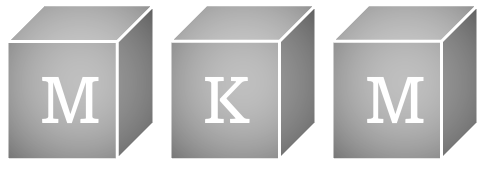
\includegraphics[width=0.4\textwidth]{../shared/Logos/MKM_logo.png}
    \end{figure}
    \vspace{1.5cm}
    {\Huge\bfseries\textcolor{mkmblue}{\doctitle}\par}
    \vspace{0.5cm}
    {\Large\textcolor{gray}{\docsubtitle}\par}
    \vspace{2cm}
    {\large MKM Research Labs\par}
    \vspace{0.5cm}
    {\large Version \docversion{} --- \docdate\par}
    \vspace{0.5cm}
    {\large \docauthor\par}
    \vspace{2cm}
    \textcolor{red}{\textbf{CONFIDENTIAL --- PROPRIETARY}}
    \end{center}
    \end{titlepage}
}

\newcommand{\mkmlegalpage}{%
    \clearpage
    \thispagestyle{empty}
    \begin{center}
    \large\textbf{Legal Notice}
    \vspace{1em}

    \textbf{PROPRIETARY AND CONFIDENTIAL}
    \end{center}

    \noindent This document, including all algorithms, models, methodology, formulas,
    calculations, and intellectual concepts contained herein, constitutes the exclusive
    intellectual property and confidential trade secrets of MKM Research Labs (``MKM'').

    \vspace{0.5em}
    \noindent Any usage, reproduction, distribution, modification, or disclosure of this
    document or any portion thereof, without the express prior written authorisation from
    MKM Research Labs is strictly prohibited and constitutes an infringement of intellectual
    property rights.

    \vspace{0.5em}
    \noindent The document is provided on an ``as is'' basis. MKM Research Labs makes no
    representations or warranties of any kind, express or implied, regarding its accuracy,
    reliability, or suitability for any particular purpose.

    \vspace{1em}
    \begin{center}
    All rights reserved. \copyright\ 2021--2026 MKM Research Labs.

    \vspace{0.5em}
    Governed by the laws of the United Kingdom.
    \end{center}
    \clearpage
}

\newcommand{\mkmhistorypage}[1]{%
    \section{Document History}
    \begin{table}[ht]
        \centering
        \begin{tabular}{l|l|l|l}
            \textbf{Date} & \textbf{Version} & \textbf{Description} & \textbf{Author} \\
            \hline
            #1
        \end{tabular}
        \label{tab:revision_history}
    \end{table}
    \clearpage
}

% ─── Bank validation protocol section commands ──────────────────────────────
% Use these to ensure every model doc has the required sections.
% They are just styled \section calls — content is provided by each doc.

\newcommand{\mkmexecsummary}{\section{Executive Summary}}
\newcommand{\mkmpurpose}{\section{Model Purpose and Scope}}
\newcommand{\mkmframework}{\section{Mathematical Framework}}
\newcommand{\mkminputs}{\section{Input Parameters and Calibration}}
\newcommand{\mkmimplementation}{\section{Implementation Details}}
\newcommand{\mkmsensitivity}{\section{Sensitivity Analysis}}
\newcommand{\mkmvalidation}{\section{Validation and Backtesting}}
\newcommand{\mkmtestresults}{\subsection{Automated Test Results}\input{test_results}}
\newcommand{\mkmlimitations}{\section{Model Limitations and Known Weaknesses}}

\newcommand{\mkmgovernance}{\section{Governance Validation Questions}
\noindent The following nine questions are mandated by Chapter~5 of the
\emph{Model Risk Governance for Vendors} handbook and must be explicitly
addressed for every model in the inventory. Response status is tracked in the
Model Governance Dashboard (MRC portal). \par\medskip}

\newcommand{\mkmvqitem}[3]{\subsection{Q#1 --- #2}
\noindent\textit{``#3''}\par\medskip\noindent}

\newcommand{\mkmchangelog}{\section{Change History}}
  (before \begin{document})
%
% Required commands before \input:
%   \newcommand{\doctitle}{...}
%   \newcommand{\docsubtitle}{...}
%   \newcommand{\docversion}{1.0}
%   \newcommand{\docdate}{13-February-2026}
%   \newcommand{\docauthor}{David K Kelly}

% ─── Packages ───────────────────────────────────────────────────────────────
\usepackage[utf8]{inputenc}
\usepackage{amsmath,amsfonts,amssymb}
\usepackage{listings}
\usepackage{color,xcolor}
\usepackage{graphicx}
\usepackage{hyperref}
\usepackage[toc,page]{appendix}
\usepackage{tabto}
\usepackage{float}
\usepackage{comment}
\usepackage[en-GB]{datetime2}
\usepackage{setspace}
\usepackage{subcaption}
\usepackage{booktabs}
\usepackage{longtable}
\usepackage{adjustbox}
\usepackage{enumitem}
\usepackage{fancyhdr}
\usepackage{lastpage}

% ─── Page geometry ──────────────────────────────────────────────────────────
\onehalfspacing
\usepackage{geometry}
\geometry{a4paper, total={170mm,247mm}, left=20mm, top=25mm, bottom=25mm}

% ─── Headers and footers ───────────────────────────────────────────────────
\pagestyle{fancy}
\fancyhf{}
\fancyhead[L]{\small\textcolor{gray}{MKM Research Labs}}
\fancyhead[R]{\small\textcolor{gray}{\doctitle{} --- v\docversion}}
\fancyfoot[C]{\small\textcolor{gray}{CONFIDENTIAL}}
\fancyfoot[R]{\small\textcolor{gray}{Page \thepage\ of \pageref{LastPage}}}
\renewcommand{\headrulewidth}{0.4pt}
\renewcommand{\footrulewidth}{0.4pt}

% ─── Colours ────────────────────────────────────────────────────────────────
\definecolor{mkmblue}{HTML}{1565C0}
\definecolor{codegreen}{rgb}{0,0.6,0}
\definecolor{codegray}{rgb}{0.5,0.5,0.5}
\definecolor{codepurple}{rgb}{0.58,0,0.82}
\definecolor{backcolour}{rgb}{0.95,0.95,0.92}

% ─── Hyperref setup ─────────────────────────────────────────────────────────
\hypersetup{
    colorlinks=true,
    linkcolor=mkmblue,
    citecolor=mkmblue,
    urlcolor=mkmblue
}

% ─── Code listings ──────────────────────────────────────────────────────────
\lstdefinestyle{mystyle}{
    backgroundcolor=\color{backcolour},
    commentstyle=\color{codegreen},
    keywordstyle=\color{magenta},
    numberstyle=\tiny\color{codegray},
    stringstyle=\color{codepurple},
    basicstyle=\ttfamily\footnotesize,
    breakatwhitespace=false,
    breaklines=true,
    captionpos=b,
    keepspaces=true,
    numbers=left,
    numbersep=5pt,
    showspaces=false,
    showstringspaces=false,
    showtabs=false,
    tabsize=2
}
\lstset{style=mystyle}

% ─── Section formatting ────────────────────────────────────────────────────
\setcounter{tocdepth}{3}
\setcounter{secnumdepth}{3}

% ─── Shared macros ──────────────────────────────────────────────────────────
\newcommand{\mkmtitlepage}{%
    \begin{titlepage}
    \begin{center}
    \vspace*{1cm}
    \begin{figure}[H]\centering
        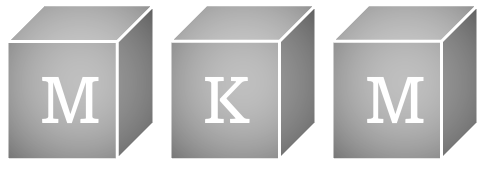
\includegraphics[width=0.4\textwidth]{../shared/Logos/MKM_logo.png}
    \end{figure}
    \vspace{1.5cm}
    {\Huge\bfseries\textcolor{mkmblue}{\doctitle}\par}
    \vspace{0.5cm}
    {\Large\textcolor{gray}{\docsubtitle}\par}
    \vspace{2cm}
    {\large MKM Research Labs\par}
    \vspace{0.5cm}
    {\large Version \docversion{} --- \docdate\par}
    \vspace{0.5cm}
    {\large \docauthor\par}
    \vspace{2cm}
    \textcolor{red}{\textbf{CONFIDENTIAL --- PROPRIETARY}}
    \end{center}
    \end{titlepage}
}

\newcommand{\mkmlegalpage}{%
    \clearpage
    \thispagestyle{empty}
    \begin{center}
    \large\textbf{Legal Notice}
    \vspace{1em}

    \textbf{PROPRIETARY AND CONFIDENTIAL}
    \end{center}

    \noindent This document, including all algorithms, models, methodology, formulas,
    calculations, and intellectual concepts contained herein, constitutes the exclusive
    intellectual property and confidential trade secrets of MKM Research Labs (``MKM'').

    \vspace{0.5em}
    \noindent Any usage, reproduction, distribution, modification, or disclosure of this
    document or any portion thereof, without the express prior written authorisation from
    MKM Research Labs is strictly prohibited and constitutes an infringement of intellectual
    property rights.

    \vspace{0.5em}
    \noindent The document is provided on an ``as is'' basis. MKM Research Labs makes no
    representations or warranties of any kind, express or implied, regarding its accuracy,
    reliability, or suitability for any particular purpose.

    \vspace{1em}
    \begin{center}
    All rights reserved. \copyright\ 2021--2026 MKM Research Labs.

    \vspace{0.5em}
    Governed by the laws of the United Kingdom.
    \end{center}
    \clearpage
}

\newcommand{\mkmhistorypage}[1]{%
    \section{Document History}
    \begin{table}[ht]
        \centering
        \begin{tabular}{l|l|l|l}
            \textbf{Date} & \textbf{Version} & \textbf{Description} & \textbf{Author} \\
            \hline
            #1
        \end{tabular}
        \label{tab:revision_history}
    \end{table}
    \clearpage
}

% ─── Bank validation protocol section commands ──────────────────────────────
% Use these to ensure every model doc has the required sections.
% They are just styled \section calls — content is provided by each doc.

\newcommand{\mkmexecsummary}{\section{Executive Summary}}
\newcommand{\mkmpurpose}{\section{Model Purpose and Scope}}
\newcommand{\mkmframework}{\section{Mathematical Framework}}
\newcommand{\mkminputs}{\section{Input Parameters and Calibration}}
\newcommand{\mkmimplementation}{\section{Implementation Details}}
\newcommand{\mkmsensitivity}{\section{Sensitivity Analysis}}
\newcommand{\mkmvalidation}{\section{Validation and Backtesting}}
\newcommand{\mkmtestresults}{\subsection{Automated Test Results}\input{test_results}}
\newcommand{\mkmlimitations}{\section{Model Limitations and Known Weaknesses}}

\newcommand{\mkmgovernance}{\section{Governance Validation Questions}
\noindent The following nine questions are mandated by Chapter~5 of the
\emph{Model Risk Governance for Vendors} handbook and must be explicitly
addressed for every model in the inventory. Response status is tracked in the
Model Governance Dashboard (MRC portal). \par\medskip}

\newcommand{\mkmvqitem}[3]{\subsection{Q#1 --- #2}
\noindent\textit{``#3''}\par\medskip\noindent}

\newcommand{\mkmchangelog}{\section{Change History}}
  (before \begin{document})
%
% Required commands before \input:
%   \newcommand{\doctitle}{...}
%   \newcommand{\docsubtitle}{...}
%   \newcommand{\docversion}{1.0}
%   \newcommand{\docdate}{13-February-2026}
%   \newcommand{\docauthor}{David K Kelly}

% ─── Packages ───────────────────────────────────────────────────────────────
\usepackage[utf8]{inputenc}
\usepackage{amsmath,amsfonts,amssymb}
\usepackage{listings}
\usepackage{color,xcolor}
\usepackage{graphicx}
\usepackage{hyperref}
\usepackage[toc,page]{appendix}
\usepackage{tabto}
\usepackage{float}
\usepackage{comment}
\usepackage[en-GB]{datetime2}
\usepackage{setspace}
\usepackage{subcaption}
\usepackage{booktabs}
\usepackage{longtable}
\usepackage{adjustbox}
\usepackage{enumitem}
\usepackage{fancyhdr}
\usepackage{lastpage}

% ─── Page geometry ──────────────────────────────────────────────────────────
\onehalfspacing
\usepackage{geometry}
\geometry{a4paper, total={170mm,247mm}, left=20mm, top=25mm, bottom=25mm}

% ─── Headers and footers ───────────────────────────────────────────────────
\pagestyle{fancy}
\fancyhf{}
\fancyhead[L]{\small\textcolor{gray}{MKM Research Labs}}
\fancyhead[R]{\small\textcolor{gray}{\doctitle{} --- v\docversion}}
\fancyfoot[C]{\small\textcolor{gray}{CONFIDENTIAL}}
\fancyfoot[R]{\small\textcolor{gray}{Page \thepage\ of \pageref{LastPage}}}
\renewcommand{\headrulewidth}{0.4pt}
\renewcommand{\footrulewidth}{0.4pt}

% ─── Colours ────────────────────────────────────────────────────────────────
\definecolor{mkmblue}{HTML}{1565C0}
\definecolor{codegreen}{rgb}{0,0.6,0}
\definecolor{codegray}{rgb}{0.5,0.5,0.5}
\definecolor{codepurple}{rgb}{0.58,0,0.82}
\definecolor{backcolour}{rgb}{0.95,0.95,0.92}

% ─── Hyperref setup ─────────────────────────────────────────────────────────
\hypersetup{
    colorlinks=true,
    linkcolor=mkmblue,
    citecolor=mkmblue,
    urlcolor=mkmblue
}

% ─── Code listings ──────────────────────────────────────────────────────────
\lstdefinestyle{mystyle}{
    backgroundcolor=\color{backcolour},
    commentstyle=\color{codegreen},
    keywordstyle=\color{magenta},
    numberstyle=\tiny\color{codegray},
    stringstyle=\color{codepurple},
    basicstyle=\ttfamily\footnotesize,
    breakatwhitespace=false,
    breaklines=true,
    captionpos=b,
    keepspaces=true,
    numbers=left,
    numbersep=5pt,
    showspaces=false,
    showstringspaces=false,
    showtabs=false,
    tabsize=2
}
\lstset{style=mystyle}

% ─── Section formatting ────────────────────────────────────────────────────
\setcounter{tocdepth}{3}
\setcounter{secnumdepth}{3}

% ─── Shared macros ──────────────────────────────────────────────────────────
\newcommand{\mkmtitlepage}{%
    \begin{titlepage}
    \begin{center}
    \vspace*{1cm}
    \begin{figure}[H]\centering
        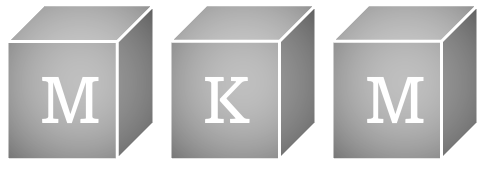
\includegraphics[width=0.4\textwidth]{../shared/Logos/MKM_logo.png}
    \end{figure}
    \vspace{1.5cm}
    {\Huge\bfseries\textcolor{mkmblue}{\doctitle}\par}
    \vspace{0.5cm}
    {\Large\textcolor{gray}{\docsubtitle}\par}
    \vspace{2cm}
    {\large MKM Research Labs\par}
    \vspace{0.5cm}
    {\large Version \docversion{} --- \docdate\par}
    \vspace{0.5cm}
    {\large \docauthor\par}
    \vspace{2cm}
    \textcolor{red}{\textbf{CONFIDENTIAL --- PROPRIETARY}}
    \end{center}
    \end{titlepage}
}

\newcommand{\mkmlegalpage}{%
    \clearpage
    \thispagestyle{empty}
    \begin{center}
    \large\textbf{Legal Notice}
    \vspace{1em}

    \textbf{PROPRIETARY AND CONFIDENTIAL}
    \end{center}

    \noindent This document, including all algorithms, models, methodology, formulas,
    calculations, and intellectual concepts contained herein, constitutes the exclusive
    intellectual property and confidential trade secrets of MKM Research Labs (``MKM'').

    \vspace{0.5em}
    \noindent Any usage, reproduction, distribution, modification, or disclosure of this
    document or any portion thereof, without the express prior written authorisation from
    MKM Research Labs is strictly prohibited and constitutes an infringement of intellectual
    property rights.

    \vspace{0.5em}
    \noindent The document is provided on an ``as is'' basis. MKM Research Labs makes no
    representations or warranties of any kind, express or implied, regarding its accuracy,
    reliability, or suitability for any particular purpose.

    \vspace{1em}
    \begin{center}
    All rights reserved. \copyright\ 2021--2026 MKM Research Labs.

    \vspace{0.5em}
    Governed by the laws of the United Kingdom.
    \end{center}
    \clearpage
}

\newcommand{\mkmhistorypage}[1]{%
    \section{Document History}
    \begin{table}[ht]
        \centering
        \begin{tabular}{l|l|l|l}
            \textbf{Date} & \textbf{Version} & \textbf{Description} & \textbf{Author} \\
            \hline
            #1
        \end{tabular}
        \label{tab:revision_history}
    \end{table}
    \clearpage
}

% ─── Bank validation protocol section commands ──────────────────────────────
% Use these to ensure every model doc has the required sections.
% They are just styled \section calls — content is provided by each doc.

\newcommand{\mkmexecsummary}{\section{Executive Summary}}
\newcommand{\mkmpurpose}{\section{Model Purpose and Scope}}
\newcommand{\mkmframework}{\section{Mathematical Framework}}
\newcommand{\mkminputs}{\section{Input Parameters and Calibration}}
\newcommand{\mkmimplementation}{\section{Implementation Details}}
\newcommand{\mkmsensitivity}{\section{Sensitivity Analysis}}
\newcommand{\mkmvalidation}{\section{Validation and Backtesting}}
\newcommand{\mkmtestresults}{\subsection{Automated Test Results}\input{test_results}}
\newcommand{\mkmlimitations}{\section{Model Limitations and Known Weaknesses}}

\newcommand{\mkmgovernance}{\section{Governance Validation Questions}
\noindent The following nine questions are mandated by Chapter~5 of the
\emph{Model Risk Governance for Vendors} handbook and must be explicitly
addressed for every model in the inventory. Response status is tracked in the
Model Governance Dashboard (MRC portal). \par\medskip}

\newcommand{\mkmvqitem}[3]{\subsection{Q#1 --- #2}
\noindent\textit{``#3''}\par\medskip\noindent}

\newcommand{\mkmchangelog}{\section{Change History}}

% T1 so the underscores in code identifiers print as underscores.
\usepackage[T1]{fontenc}
\usepackage{lmodern}
% Generated by tools.wolfram_oracle -- do not edit.
\newcommand{\bmGenerated}{2026-11-04}
\newcommand{\bmCodeCommit}{\texttt{bf0c281bd086}}
\newcommand{\bmCodeDirty}{}
\newcommand{\bmNumerics}{numpy 1.26.4, scipy 1.15.1, mpmath 1.4.1}
\newcommand{\bmWolfram}{15.0.0 for Mac OS X ARM (64-bit) (May 26, 2026)}
\newcommand{\bmWolframVia}{ via live kernel session (wolframclient)}
\newcommand{\bmWolframConfirms}{Wolfram, computing each independently, agrees with the reference to $4.5\times10^{-31}$.}
\newcommand{\bmChecks}{8}
\newcommand{\bmOutcome}{all pass}
\newcommand{\bmCodeErr}{$9.4\times10^{-15}$}
\newcommand{\bmLevelErr}{$4.4\times10^{-14}$}
\newcommand{\bmRuns}{780}
\newcommand{\bmClaims}{16}
\newcommand{\bmClaimsMet}{16}
\newcommand{\bmFigures}{169}

% The shared history table sets every column to its natural width; wrap the description.
\renewcommand{\mkmhistorypage}[1]{%
    \section{Document History}
    \begin{table}[ht]
        \centering
        \begin{tabular}{l|l|p{9cm}|l}
            \textbf{Date} & \textbf{Version} & \textbf{Description} & \textbf{Author} \\
            \hline
            #1
        \end{tabular}
    \end{table}
}

\begin{document}
% Long code paths and identifiers cannot hyphenate; let the spacing stretch instead.
\sloppy

\mkmtitlepage
\mkmlegalpage

\tableofcontents
\clearpage

% =========================================================================
\mkmexecsummary
% =========================================================================

This document benchmarks the Storm-Gauge Forward Model (MKM-SG-001): the package
\texttt{src/models/stormgauge/}, which turns a storm's track, intensity and footprint
into a water level at each gauge. It asks whether the code computes what its model
document (\texttt{storm\_gauge.pdf}, v1.3 of 11 March 2026, as filed) says, and whether
what the document says holds.

\paragraph{The code computes its documented equations.} The haversine, the track
interpolation, the three decay kernels, the intensity at the gauge and the power law
agree with a 50-digit implementation of the document's equations to \bmCodeErr. Over
\bmRuns{} runs of the full response (Eqs.~14--18), the water level agrees to
$2\times10^{-14}$\,m, and every peak time and duration is identical
(Table~\ref{tab:bm-checks}). \bmWolframConfirms{} That includes Wolfram's own
implementation of the whole response, written separately from the reference.

\paragraph{The document's account of the model does not hold:} \bmClaimsMet{} of
\bmClaims{} claims are met (Table~\ref{tab:bm-claims}). What holds is the arithmetic: all
\bmFigures{} figures in its four sensitivity tables reproduce, as do its kernel
percentages, its calibration targets read as Eq.~13's steady state, and its timings.
What does not hold is what the model is said to do, and where its output is said to go.
\begin{itemize}[leftmargin=*,nosep]
\item \textbf{Nothing uses it.} Section~2.2 and Q5--Q6 say the model's responses fill
  \texttt{gaugets/} and feed the hazard curves, the flood risk model and MKM-TS-001.
  Nothing in \texttt{src}, \texttt{tools} or \texttt{scripts} imports the package.
  \texttt{gaugets/} is written by a scripted flood wave, not by this model.
\item \textbf{A storm does not reach the levels the calibration names.} The targets
  of \S3.5 (alert at $I\approx40$, severe at 85+) hold only for a level held at Eq.~13's
  target indefinitely. A default storm crossing the gauge needs a peak of 56 to reach
  alert and 94 to reach warning, and does not reach severe at all.
\item \textbf{The dynamics are not as described.} Peak level follows peak intensity
  by 3.5--5\,h, not $\tau_{\mathrm{lag}}=2$\,h. Doubling $\tau_{\mathrm{decay}}$ lowers
  the peak by 19\% and shortens the time above alert, rather than doubling it. The run
  ends with the storm, so durations and accumulation stop counting while the gauge is
  still high.
\item \textbf{Two of its inputs are unread:} the intensity-to-level scale, whose
  Table~5 has six identical rows, and the storm's speed.
\item \textbf{Two figures are overstated:} the effect of $\gamma$ (\S6.2), and the
  sphere's accuracy at UK scale, which is 0.32\%, not under 0.3\%.
\end{itemize}

\paragraph{Evidence.} \bmChecks{} checks, outcome: \bmOutcome{}
(Table~\ref{tab:bm-checks}).
\begin{itemize}[leftmargin=*,nosep]
\item Wolfram: \bmWolfram{}\bmWolframVia.
\item Code under test, at commit \bmCodeCommit{}\bmCodeDirty.
\item Numerics: \bmNumerics.
\item Generated \bmGenerated{} by \texttt{python -m tools.wolfram\_oracle sg001}.
\end{itemize}

% =========================================================================
\mkmpurpose
% =========================================================================

\subsection{What is benchmarked}
The package v1.3 documents, imported as its own tests import it:
\begin{itemize}[leftmargin=*,nosep]
\item \texttt{forward\_model.StormGaugeModel}: the haversine, the decay kernels, the
  intensity at a gauge, the power law, and \texttt{compute\_response}, which produces
  the level series and its statistics;
\item \texttt{storm\_factory.create\_storm}, which builds the storms the cases use;
\item \texttt{data\_structures}: the storm, gauge and response types.
\end{itemize}

\subsection{What is not}
\begin{itemize}[leftmargin=*,nosep]
\item The calibration of $\gamma$, $\tau_{\mathrm{lag}}$ and $\tau_{\mathrm{decay}}$
  to Environment Agency records (\S4.4), and the backtest of \S7.2, which are
  empirical. Nothing in the repository runs the model against gauge records, so
  neither can be reproduced from it.
\item \texttt{find\_nearest\_track\_point}, which \texttt{compute\_response} does not
  call.
\item The scripted wave that does write \texttt{gaugets/}
  (\texttt{port/rand/shared/gauge/gaugets\_random}), and MKM-SS-001's sequence
  response, which re-implements Eq.~16 rather than calling this code.
\end{itemize}
This is a benchmark of the implementation (validation question Q8), not independent
validation (Q9).

% =========================================================================
\mkmframework
% =========================================================================

The reference implements v1.3's equations directly from its text:
\begin{itemize}[leftmargin=*,nosep]
\item the haversine of Eqs.~1--2, in its arctangent form, on a sphere of 6{,}371\,km;
\item the track interpolation of Eqs.~3--6, with $\alpha$ clamped to $[0,1]$;
\item the Gaussian, exponential and linear kernels of Eqs.~7--10, with $k=1$ on the
  track;
\item the intensity at the gauge, $I_s(t)\,k(\tilde d(t))$ (Eq.~11);
\item the power law $\Delta L=(I/100)^{0.8}L_{\mathrm{range}}\,s$ of Eqs.~12--13,
  with $L_{\mathrm{high}}=1.1L_{\mathrm{severe}}$ where a gauge has no historical high;
\item the response of Eqs.~14--16 on \S5.2's grid $t_i=i\,\Delta t$,
  $i=0,\ldots,\lfloor T/\Delta t\rfloor$: the target is Eq.~13 at the intensity
  $\lfloor\tau_{\mathrm{lag}}/\Delta t\rfloor$ steps earlier, approached at rate
  $\min(1,3\Delta t/\tau_{\mathrm{decay}})$ when rising and $\Delta t/\tau_{\mathrm{decay}}$
  when falling;
\item the peaks, the durations of Eq.~17 and the accumulation of Eq.~18.
\end{itemize}

\paragraph{Where the document is silent,} the reference assumes what the code does.
Before the first track point the storm sits at it, and after the last at the last.
Before $\tau_{\mathrm{lag}}$ has elapsed, Eq.~15 reads the first step. The cases
exercise both: one track starts late, and the Gaussian profile does not start at zero.

% =========================================================================
\section{Benchmark Method}
% =========================================================================

\paragraph{The cases.}
\begin{itemize}[leftmargin=*,nosep]
\item A default storm (Table~1: 24\,h, 25 track points, footprint 40\,km, triangular
  profile, Gaussian kernel at 0.5) crosses the Thames west to east, at peaks of 30,
  50, 80 and 100.
\item The same storm with every other kernel and profile, and an irregular storm whose
  track starts late, turns and ends early.
\item Five gauges: on the track, 0.1, 0.2 and 0.4$^\circ$ north of it, and one with a
  historical high and a sensitivity of 1.3.
\item Four settings of $(\Delta t,\tau_{\mathrm{lag}},\tau_{\mathrm{decay}})$, one
  with a lag that is not a whole number of steps; and durations of 24, 23.7 and 48\,h.
\end{itemize}
The closed-form families also run on distances and intensities below zero, at zero,
and far beyond the footprint.

\paragraph{The printed tables.} Tables~4 and~5 were produced by the house sensitivity
generator; each figure is judged as the code's value, rounded and formatted as that
generator does. Tables~6 and~7 were written by hand, and are judged to the places they
print.

\paragraph{The statements.} Each statement about the model's behaviour is judged by
running the code, which the checks show computes the document's equations.
\begin{itemize}[leftmargin=*,nosep]
\item The calibration targets are solved twice: from Eq.~13 directly, and as the least
  peak intensity at which a default storm crossing the gauge reaches each stage.
\item The lag is measured over every case in which the gauge feels the storm.
\item $\tau_{\mathrm{decay}}$ and $\tau_{\mathrm{lag}}$ are doubled on the peak-100
  crossing.
\item The durations are compared with the same storm run on to 72\,h.
\item An input is unread if changing it changes no response.
\item Where the output goes is found by searching the tree for anything that imports
  the package.
\end{itemize}

\paragraph{Wolfram.} Wolfram works from each input's exact value, independently of the
reference:
\begin{itemize}[leftmargin=*,nosep]
\item the great-circle distance, as $R$ times the angle between the two points' unit
  vectors (not the haversine);
\item the kernels and the power law;
\item the whole response, written again in the Wolfram Language for three storms (the
  default crossing, an exponential storm with a beta profile off the track, and the
  irregular storm), returning the peak level, the accumulation and the final level;
\item the true distance between six UK pairs, by \texttt{GeoDistance} on WGS84.
\end{itemize}

% =========================================================================
\mkmvalidation
% =========================================================================

% Generated by tools.wolfram_oracle -- do not edit.
\begin{table}[H]\centering\small
\caption{Benchmark checks}\label{tab:bm-checks}
\begin{adjustbox}{max width=\textwidth}
\begin{tabular}{p{96mm}p{16mm}rl}
\toprule
Check & Result & Limit & Outcome \\
\midrule
Eqs.~1--2, the haversine: code against the reference, worst error (m) & $9.0\times10^{-10}$ & $1.0\times10^{-6}$ & pass \\
Eqs.~7--10, the decay kernels: code against the reference, worst relative error & $9.8\times10^{-16}$ & $1.0\times10^{-12}$ & pass \\
Eqs.~3--6 and 11, the intensity at the gauge: code against the reference, worst relative error & $9.4\times10^{-15}$ & $1.0\times10^{-12}$ & pass \\
Eqs.~12--13, the intensity-to-level power law: code against the reference, worst relative error & $8.1\times10^{-16}$ & $1.0\times10^{-12}$ & pass \\
Eqs.~14--16, the response and its recession over 780 runs: worst level error (m) & $4.4\times10^{-14}$ & $1.0\times10^{-6}$ & pass \\
\S3.7, peak level, peak intensity and accumulation (Eq.~18): worst relative error & $5.7\times10^{-14}$ & $1.0\times10^{-12}$ & pass \\
\S3.7, peak times and durations (Eq.~17): statistics that differ & 0 & 0 & pass \\
Wolfram agrees with the reference & $4.5\times10^{-31}$ & $1.0\times10^{-25}$ & pass \\
\bottomrule
\end{tabular}
\end{adjustbox}
\end{table}


\subsection{The model document's claims}
% Generated by tools.wolfram_oracle -- do not edit.
\begin{table}[H]\centering\small
\caption{The model document's claims, tested}\label{tab:bm-claims}
\begin{adjustbox}{max width=\textwidth}
\begin{tabular}{p{20mm}p{52mm}p{64mm}l}
\toprule
Claim & Stated & Benchmark finds & Outcome \\
\midrule
\S3.3.1 & Gaussian: 60.7\% of on-track intensity at $\tilde d=\sigma$, 13.5\% at $2\sigma$ & as printed & met \\
Table~4 & decay by kernel and distance & 21 of 21 figures reproduced & met \\
Table~5 & contribution by intensity and scale factor & 30 of 30 figures reproduced & met \\
Table~6 & $k(1.0)$ for each kernel & 3 of 3 figures reproduced & met \\
Table~7 & $(1/2)^\gamma$ for four exponents & 4 of 4 figures reproduced & met \\
Tables~1, 5 & the scale factor and the storm's speed are model inputs & changing either changes nothing; Table~5's six rows are identical & \textbf{not met} \\
\S6.2 & $\pm$25\% in $\gamma$ moves a mid-range contribution by 20--25\% & +14.9\% and -12.9\% at $I=50$; 9.7\%--20.1\% over $I=40$--60 & \textbf{not met} \\
\S3.5 & the level reaches alert at $I\approx40$, warning at 60--70, severe at 85+, the high at 100 & Eq.~13's target does: at 38.7, 64.7, 86.0 and 100 & met \\
\S3.5 & \ldots and so does a storm of that intensity & a default storm crossing the gauge reaches alert at peak 56.0, warning at 93.6, severe never, even at 100 & \textbf{not met} \\
\S3.7, \S7.1 & peak level follows peak intensity by about $\tau_{\mathrm{lag}}=2$\,h & by 3.5 to 5.0\,h & \textbf{not met} \\
\S6.3 & doubling $\tau_{\mathrm{decay}}$ roughly doubles the time above alert; peak barely moves & 12.0\,h becomes 9.5\,h; the peak moves -18.8\% & \textbf{not met} \\
\S6.3 & a longer $\tau_{\mathrm{lag}}$ moves the timing, not the peak & doubled, the peak moves +0.0\% and +2.0\,h & met \\
\S3.7 & durations are the total time above each stage & the run stops at the storm's end, the level still 2.84\,m up (68.7\% of its rise); run on, 12.0\,h above alert becomes 13.0\,h & \textbf{not met} \\
\S8(5) & the sphere is within 0.3\% of the ellipsoid at UK scale & -0.32\% to -0.06\% against \texttt{GeoDistance} on WGS84 & \textbf{not met} \\
Q3 & under 10\,ms a gauge; 25 gauges under 250\,ms & 0.3\,ms; 6\,ms & met \\
\S2.2, Q5, Q6 & its responses fill \texttt{gaugets/} and feed the hazard curves, MKM-PF-001 and MKM-TS-001 & nothing in \texttt{src}, \texttt{tools} or \texttt{scripts} imports it & \textbf{not met} \\
\bottomrule
\end{tabular}
\end{adjustbox}
\end{table}


\subsection{What the findings mean}

\paragraph{The model is not on any production path.} The document places it at the
centre of the chain: its responses stored in \texttt{gaugets/}, consumed by the hazard
curves, the flood risk model and the time-series statistics (\S2.2, Q5, Q6). No module
imports \texttt{models.stormgauge}. \texttt{gaugets/} is written by
\texttt{port/src/gauge/gaugets.py} from \texttt{gaugets\_random}, a scripted wave with
staggered peaks and a sinusoidal ripple. So the governance record describes as
production a model that produces nothing. The code is correct; the record of where it
is used is not.

\paragraph{The calibration describes a steady state no storm reaches.} Eq.~16 closes
only $3\Delta t/\tau_{\mathrm{decay}}=12.5\%$ of the gap to its target each half-hour.
A triangular storm's target falls again long before the level arrives: the peak-100
crossing rises to 74\% of its target. The intensity bands of \S3.5 are therefore
Eq.~13's, not the model's. A storm must be far stronger than the bands say to reach
each stage.

\paragraph{The same smoothing explains the lag, $\tau_{\mathrm{decay}}$ and the
durations.}
\begin{itemize}[leftmargin=*,nosep]
\item The level keeps rising for as long as the falling target is still above it.
  That adds 1.5--3\,h to the 2\,h lag. No unit test checks the lag, although \S7.1
  says one does.
\item $\tau_{\mathrm{decay}}$ sets the rise as well as the fall. Doubling it halves
  the rising rate, and so lowers the peak, before it lengthens anything.
\item The grid stops at $T$ (\S5.2). At the end of the peak-100 crossing the gauge is
  still 2.84\,m above base, 69\% of its rise, and above alert. Run on, it stays above
  alert another hour.
\end{itemize}

\paragraph{The smaller findings.}
\begin{itemize}[leftmargin=*,nosep]
\item \texttt{intensity\_to\_level\_scale} is stored and never read; Table~5's caption
  presents it as a sensitivity, and its rows are identical. The storm's
  \texttt{speed\_kmh} is computed and never read.
\item A $\pm$25\% change in $\gamma$ moves the contribution at $I=50$ by +14.9\% and
  $-$12.9\%, and by 10--20\% across $I=40$--60, not 20--25\%.
\item The sphere understates the default storm's own east--west track by 0.32\%,
  slightly more than \S8(5)'s 0.3\%; north--south it errs by 0.06\%. That is
  immaterial beside the findings above.
\end{itemize}

% =========================================================================
\mkmlimitations
% =========================================================================

\begin{enumerate}[leftmargin=*]
\item \textbf{Benchmark, not validation.} The code is shown to compute its documented
  equations. Whether $\gamma=0.8$ and the time constants fit UK catchments is an
  empirical question, and nothing in the repository tests it.
\item \textbf{The claims are judged on the code's defaults.} Every behavioural claim
  is judged on Table~1's default storm and Table~2's default gauge. A gauge with its own
  historical high moves the steady-state bands. It does not change the smoothing that
  keeps a storm from reaching them.
\end{enumerate}

\mkmhistorypage{04-Nov-2026 & 0.1 & First issue: tests the filed v1.3 & David K Kelly \\}

\end{document}
